Due to the restricted amount of memory on the GPU deep learning models cannot have a high-resolution image as their input in the scope of this research. Yet this is also not obligatory: as the image contains dozens of cells within it, its processing can be limited to a crop of a smaller size. After the model has predicted fluorescence signal for each of the crops, output fluorescence images can be combined together to form a high-resolution image again. In this thesis the architecture of the model assumes an input size of $(256, 256)$ or more specifically $(None, 1, 256, 256)$, where the first dimension is responsible for the batch size and the second one states that the input is a 1-channel image. 

There are several ways of how one can split the image, the easiest approach would be to use a sliding window of size $w$. This algorithm is depicted in Figure \ref{fig:sliding-window}. A small window starts sliding the image from the upper left to the lower right corner with step size $s$ feeding the selected crops into a deep learning model. From the output of the model only a center part of such a crop is accepted to form a full fluorescence image. Border size $b$ in this case is the size of the edges of the crop that are not accepted from the predictions of the deep learning model.

Accepted areas from each of the crops have to follow each other without any space in between. In oder to achieve that if the border size has been defined in advance, one has to set the step size to in the following way:
\begin{equation}
  s = w - 2 * b
\end{equation}
When step size $s$ is equal to window size $w$, there is no overlap between the windows.

\begin{figure}[htb]
	\begin{center}
		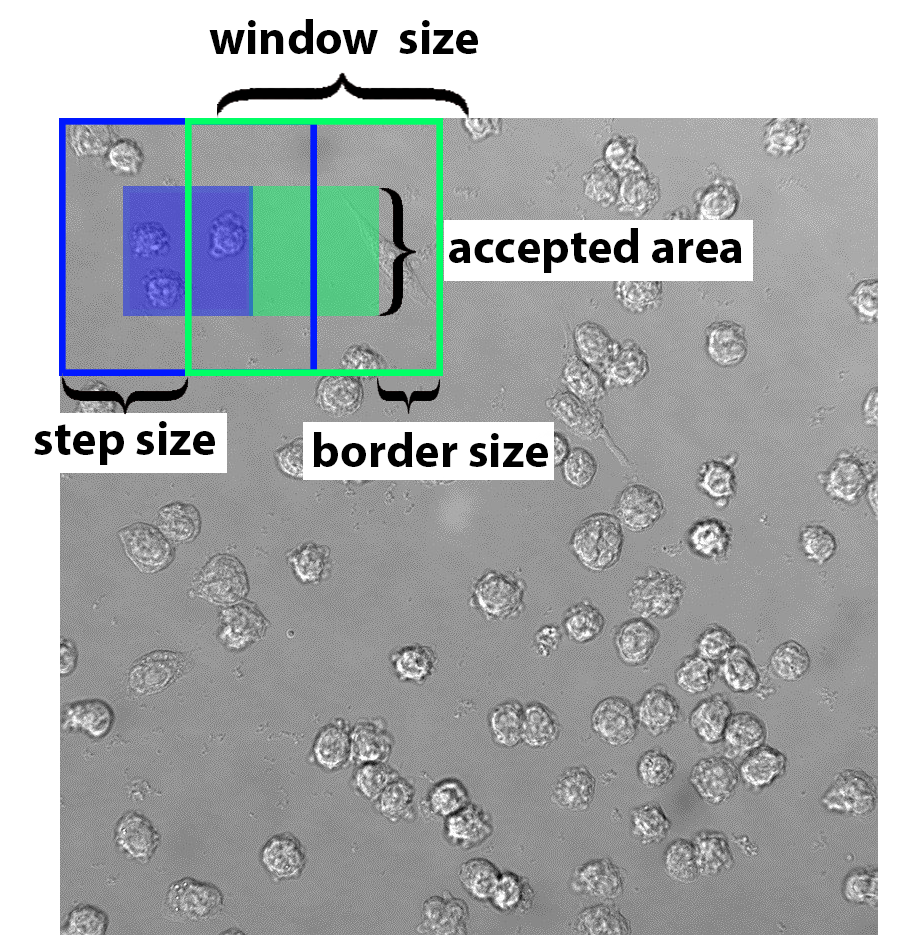
\includegraphics[width=0.4\linewidth]{bilder/sliding-window.png}
		\caption[Sliding window approach for fluorescence prediction]%
		{Sliding window approach for fluorescence prediction. Instead of predicting each crop from the image subsequently overlapping crops are used with only the center area being accepted. The size of the not accepted area is defined by a \textit{border size} value. Having a fixed \textit{window size} (defined by a neural network input), the \textit{step size} is defined dynamically.}\label{fig:sliding-window}
	\end{center}
\end{figure}
The reason why the full prediction is not accepted to form the output lies in the following: trained models are less accurate on the borders of the crops rather than in the center. Most of the times there are cells on the borders of the crops that were sliced and therefore it might be impossible to make a good prediction for them just due to the lack of input information. Therefore, the step size has to be smaller than the window size, so that the windows are overlapping and for each prediction we use only the image center and are allowed to ignore predictions on the border (see the comparison between different border sizes in Figure \ref{fig:crops-combination}). Such an approach helps to reduce the effect of grid visibility on the image composed of many small crops. This can be seen in the left part of Figure 5 as opposed to the non-visible borders in the same Figure on the right. This would of course take more time to created the predictions, however, the speed is less crucial in comparison to the accuracy of the predictions.

\begin{figure}[htb]
	\begin{center}
		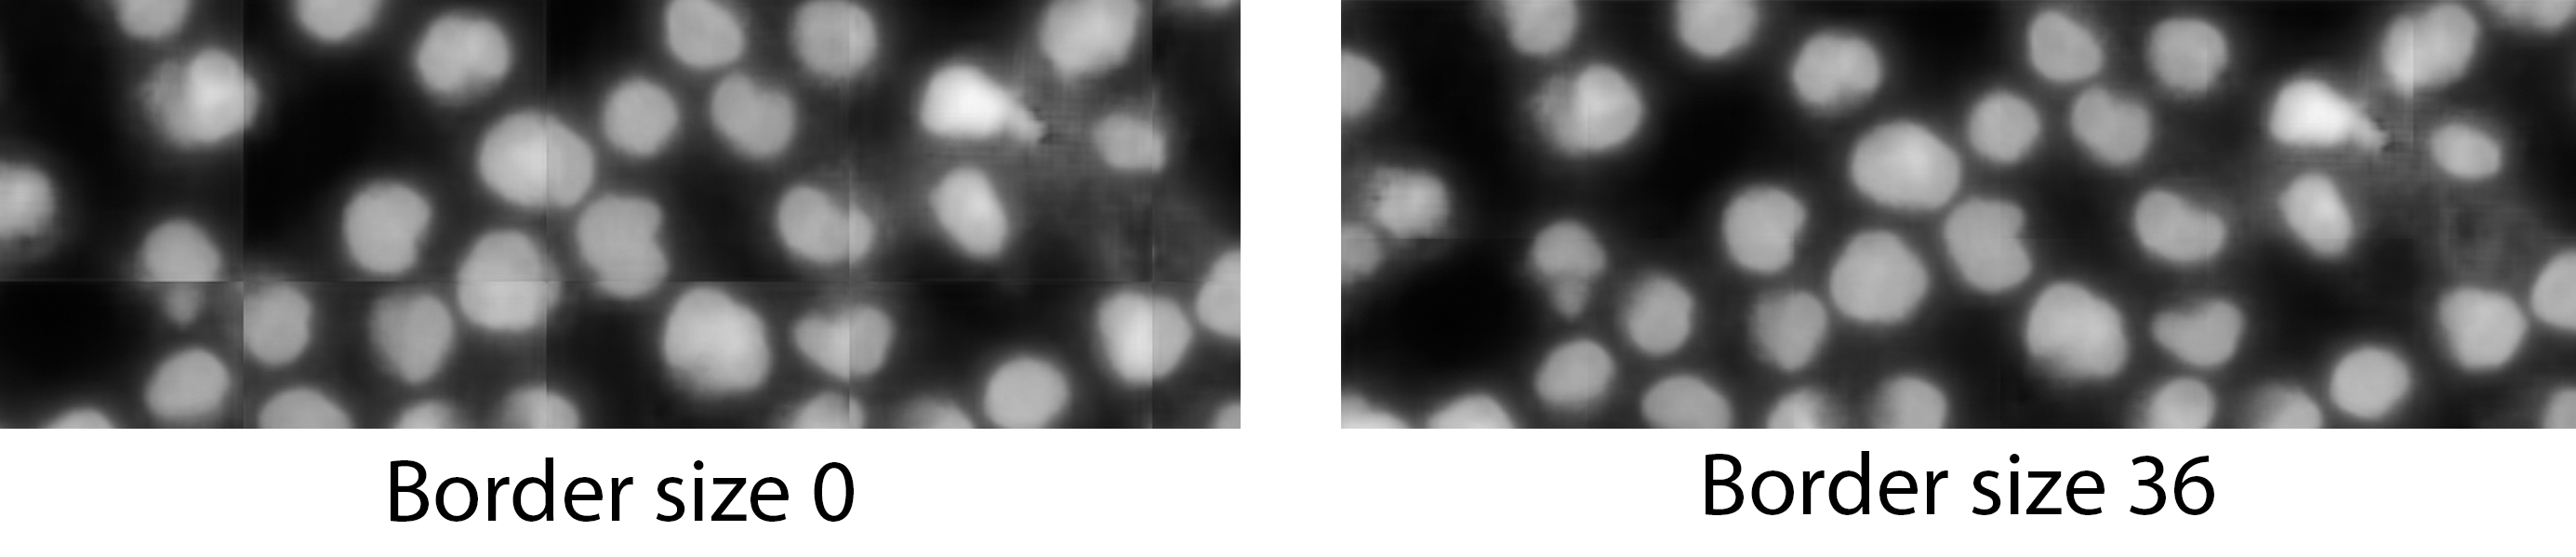
\includegraphics[width=\linewidth]{bilder/crops_combination/crops-combination.png}
		\caption[Difference of overlap between predictions on the resulting image]%
		{Difference of overlap between predictions on the resulting image. Since predictions tend to give better results in center of the crops, combination of overlapping prediction (right, with not accepted border of size $36$ pixels) results in a visually better overall image rather then combination of predictions without any overlaps (left, the whole crop is accepted). Crops intersections are highlighted in green: strongly visible on the left, and almost invisible on the right.}\label{fig:crops-combination}
	\end{center}
\end{figure}